\documentclass[10pt, a4paper]{article}

% --- Sprache & Encoding ---
\usepackage[T1]{fontenc}
\usepackage[utf8]{inputenc}
\usepackage[ngerman]{babel}
\usepackage[german=swiss]{csquotes}

% --- Layout ---
\usepackage[
    left=2.5cm,
    right=2.5cm,
    top=2.5cm,
    bottom=2.5cm
]{geometry}

% --- Grafiken ---
\usepackage{graphicx}
\usepackage{float}

% --- Mehrspaltig ---
\usepackage{multicol}
\raggedcolumns

% --- Listen ---
\usepackage{enumitem}

% --- Anpassung der Überschriften (Wichtig für Platzersparnis) ---
\usepackage{titlesec}
\titlespacing*{\section}{0pt}{2ex plus 1ex minus .2ex}{1ex plus .2ex}
\titlespacing*{\subsection}{0pt}{1.5ex plus 0.5ex minus .2ex}{0.5ex plus .2ex}

% --- Absatzformatierung ---
\setlength{\parindent}{0pt}
\setlength{\parskip}{0.2em} % Leicht reduziert für mehr Kompaktheit

% --- Seitenumbruch-Qualität ---
\widowpenalty=10000
\clubpenalty=10000
\displaywidowpenalty=10000

\begin{document}

% --- TITELBLATT ---
\begin{titlepage}
    \centering
    \vspace*{4cm}
    {\Huge \textbf{Strukturvalidierung eines systemdynamischen Modells zur Landnutzungsdynamik in den EU27 (2026–2050)}\par}
    \vspace{1.5cm}
    {\Large Expert Briefing Document\par}
    
    \vspace{4cm}
    % PLATZHALTER FÜR AUTOREN
    {\large \textbf{Autoren:}\\
    Roberto Fazekas\\
    Alexis Boser Makaratzis\par}
    
    \vfill
    {\large \today\par}
\end{titlepage}

\newpage

% --- HAUPTDOKUMENT ---
\small

Wir sind zwei Data-Science-Studierende der FHNW mit einem besonderen Interesse an der Modellierung komplexer Systeme. Im Rahmen eines systemdynamischen Modellierungsprojekts untersuchen wir die strukturelle Wechselwirkung zwischen Urbanisierungsprozessen und landwirtschaftlicher Flächennutzung in den EU27 im Zeitraum 2026–2050.

Mit einem systemdynamischen Ansatz haben wir ein erstes konzeptionelles Modell entwickelt, das zentrale Zusammenhänge zwischen wirtschaftlichem Wachstum, Flächenverbrauch, landwirtschaftlicher Produktion sowie politischen Steuerungsmechanismen strukturiert abbildet. Unsere Arbeit versteht sich ausdrücklich als explorativer Beitrag mit dem Ziel, potenzielle Rückkopplungsstrukturen und systemische Dynamiken sichtbar zu machen.

\section*{1. Zielsetzung der Anfrage}

Ziel dieser Anfrage ist nicht die Validierung von Simulationsergebnissen oder Parametrisierungen, sondern die Strukturvalidierung der angenommenen kausalen Mechanismen auf konzeptioneller Ebene.

Wir möchten prüfen,
\begin{itemize}[itemsep=0pt, topsep=0pt, leftmargin=*]
    \item ob die modellierten Einflussbeziehungen fachlich plausibel sind
    \item ob relevante Mechanismen fehlen
    \item ob die angenommene Wirkungsrichtung konsistent mit dem Stand der Literatur ist
    \item und ob zentrale Rückkopplungsstrukturen adäquat abgebildet sind
\end{itemize}

\section*{2. Modellrahmen und Systemgrenzen}
Das Modell aggregiert die EU27 als makroskopisches Gesamtsystem. Regionale Differenzierungen werden in dieser Phase nicht modelliert.

Der Simulationszeitraum umfasst 2026–2050. Historische Daten (2000–2025) dienen der konzeptionellen Kalibrierung.

Die Modellierung basiert auf einem strukturellen Ansatz der System Dynamics, bei dem die Dynamik des Systems durch endogene Rückkopplungsstrukturen beschrieben wird.

Nicht modelliert werden:
\begin{itemize}[itemsep=0pt, topsep=0pt, leftmargin=*]
    \item explizite Klimadynamiken
    \item geopolitische Schocks
    \item globale Marktdynamiken
\end{itemize}

\section*{3. Zentrale Annahmen}
\begin{itemize}[itemsep=0pt, topsep=0pt, leftmargin=*]
    \item Aggregation über EU27 ist strukturell zulässig
    \item Land Conversion beschreibt primär die Umwandlung landwirtschaftlicher Fläche
    \item Bevölkerung wirkt exogen auf Wohnraumnachfrage
    \item Beziehungen werden als monoton gerichtet modelliert
    \item Rückumwandlungsprozesse (Urban → Agricultural) werden nicht als dominanter Trend angenommen
\end{itemize}
Diese Annahmen sind explizit dokumentiert und offen zur Diskussion.

\section*{4. Konkrete Fragen an die Expert:innen}
\begin{enumerate}[itemsep=2pt, topsep=0pt, leftmargin=*]
    \item Ist der Fokus auf das Wechselspiel zwischen Landwirtschfsfläche und Urbaner Fläche bezüglich Landnutzungsdynamiken korrekt?
    \item Sind die identifizierten Kernmechanismen relevant und korrekt?
    \item Sind die identifizierten Kernmechanismen vollständig oder fehlen strukturell relevante Einflussfaktoren?
    \item Sind die angenommenen Wirkungsrichtungen fachlich konsistent?
    \item Gibt es bekannte Nichtlinearitäten oder Schwellenwerte, die strukturell berücksichtigt werden sollten?
    \item Sind relevante zeitliche Verzögerungen konzeptionell falsch eingeschätzt?
    \item Gibt es aus Ihrer Sicht weitere übergeordnete Aspekte oder alternative strukturelle Erklärungsansätze, die wir bei der Validierung prüfen sollten?
\end{enumerate}

% --- CLD Bild ---
\begin{figure}[H]
    \centering
    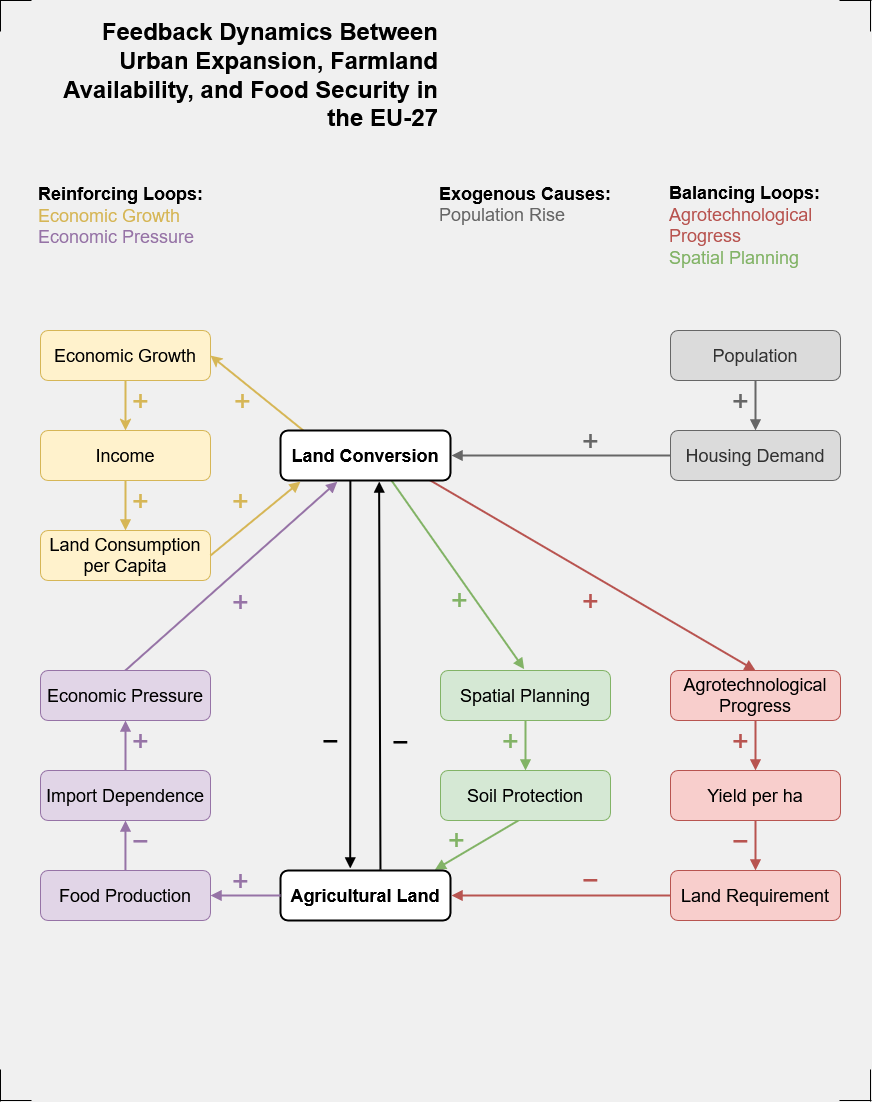
\includegraphics[width=1.0\textwidth]{./documentation-cld/assets/cld.png}
    \caption{Causal Loop Diagram (CLD) der Systemarchitektur des Modells}
\end{figure}

\newpage
\section*{5. Dokumentation pro Loop}
\vspace{0.2cm}

% --- Loops in 2x2 Layout ---
\begin{multicols}{2}

\subsection*{Reinforcing Loop 1 (Violett):\\ Import Pressure}
Sinkende Produktion aufgrund von Land Conversion führt zu erhöhter Importabhängigkeit. Der daraus resultierende ökonomische Druck verstärkt Land Conversion.

Land Conversion $\rightarrow$ Agricultural Land $\rightarrow$ Food Production $\rightarrow$ Import Dependence $\rightarrow$ Economic Pressure $\rightarrow$ Land Conversion

\vspace{0.4cm}

\subsection*{Reinforcing Loop 2 (Gelb):\\ Economic Growth}
Land Conversion fördert wirtschaftliches Wachstum, erhöht die Flächennachfrage und verstärkt dadurch wiederum Land Conversion.

Economic Growth $\rightarrow$ Income $\rightarrow$ Land Consumption per Capita $\rightarrow$ Land Conversion $\rightarrow$ Economic Growth

\columnbreak

\subsection*{Balancing Loop 1 (Rot):\\ Agricultural Technology}
Agrotechnologischer Fortschritt erhöht den Ertrag pro Hektar und reduziert bei gegebener Produktion den Flächenbedarf.

Land Conversion $\rightarrow$ Agrotechnological Progress $\rightarrow$ Yield per ha $\rightarrow$ Land Requirement $\rightarrow$ Agricultural Land $\rightarrow$ Land Conversion

\vspace{0.4cm}

\subsection*{Balancing Loop 2 (Grün):\\ Spatial Planning}
Abnehmende landwirtschaftliche Fläche kann politische Intervention auslösen, wodurch Raumplanung und Bodenschutz Land Conversion dämpfen.

Land Conversion $\rightarrow$ Spatial Planning $\rightarrow$ Soil Protection $\rightarrow$ Agricultural Land $\rightarrow$ Land Conversion

\end{multicols}

\vspace{0.5cm}

\section*{6. Dokumentation pro Beziehung im CLD}
\vspace{0.2cm}

\footnotesize % Noch etwas kleiner für maximale Kompaktheit
\begin{multicols}{2}

% --- Block 1 ---
\begin{minipage}{\linewidth}
\subsection*{Land Conversion $\rightarrow$ Agricultural Land}

\textbf{Wirkungslogik:}\\
Die Umwandlung von Land in Siedlungsfläche reduziert direkt die verfügbare landwirtschaftliche Fläche.
Agricultural Land wird als Bestandsvariable modelliert, deren Umfang durch Flächenumwandlungen reduziert wird.
Die Beziehung wird als monoton fallend modelliert.

\textbf{Zeit:}\\
Direkte Wirkung nach Umsetzung der Landnutzungsänderung.

\textbf{Annahmen:}\\
Rückumwandlung ist strukturell nicht dominant.
\end{minipage}\vspace{1em}

% --- Block 2 ---
\begin{minipage}{\linewidth}
\subsection*{Agricultural Land $\rightarrow$ Land Conversion}

\textbf{Wirkungslogik:}\\
Die verfügbare landwirtschaftliche Fläche beeinflusst die Flächenumwandlung über Knappheits- und Schutzmechanismen.
Bei abnehmender landwirtschaftlicher Fläche steigt deren wahrgenommene Knappheit und gesellschaftliche Bedeutung, was politische und regulatorische Massnahmen zur Begrenzung weiterer Umnutzung begünstigen kann.
Die Beziehung wird als monoton fallend modelliert.

\textbf{Zeit:}\\
Verzögerte Wirkung durch politische Entscheidungsprozesse und institutionelle Anpassungen.

\textbf{Annahmen:}\\
Flächenknappheit führt zu verstärktem Schutz landwirtschaftlicher Flächen.
\end{minipage}\vspace{1em}

% --- Block 3 ---
\begin{minipage}{\linewidth}
\subsection*{R1: Agricultural Land $\rightarrow$ Food Production}

\textbf{Wirkungslogik:}\\
Mehr landwirtschaftliche Fläche erhöht bei konstantem Ertrag die mögliche Nahrungsmittelproduktion.
Food Production wird als Funktion der landwirtschaftlichen Fläche und des Flächenertrags modelliert. \\
Die Beziehung wird als monoton steigend modelliert.

\textbf{Vorzeichen:} +

\textbf{Zeit:}\\
Produktionsverzögerung durch landwirtschaftliche Zyklen.

\textbf{Annahmen:}\\
Produktion proportional zur Fläche bei gegebenem Ertrag.
\end{minipage}\vspace{1em}

% --- Block 4 ---
\begin{minipage}{\linewidth}
\subsection*{R1: Food Production $\rightarrow$ Import Dependence}

\textbf{Wirkungslogik:}\\
Sinkende heimische Nahrungsmittelproduktion erhöht die Abhängigkeit von Importen.
Import Dependence wird als Funktion der Differenz zwischen inländischer Produktion und Nachfrage interpretiert.

\textbf{Zeit:}\\
Kurzfristige Anpassung über Handelsmärkte.

\textbf{Annahmen:}\\
Die EU ist kein vollständig autarkes Ernährungssystem.
\end{minipage}\vspace{1em}

% --- Block 5 ---
\begin{minipage}{\linewidth}
\subsection*{R1: Import Dependence $\rightarrow$ Economic Pressure}

\textbf{Wirkungslogik:}\\
Steigende Importabhängigkeit erzeugt wirtschaftlichen Druck. Import Dependence wird im Modell als Indikator für Versorgungssicherheit interpretiert.
Steigende Importabhängigkeit kann wirtschaftlichen oder politischen Druck erzeugen, die heimische Produktion oder wirtschaftliche Aktivität zu steigern.\\
Die Beziehung wird als monoton steigend modelliert.

\textbf{Zeit:}\\
Mittelfristige politische und wirtschaftliche Anpassungsprozesse.

\textbf{Annahmen:}\\
Importabhängigkeit wird politisch und ökonomisch als Problem wahrgenommen.
\end{minipage}\vspace{1em}

% --- Block 6 ---
\begin{minipage}{\linewidth}
\subsection*{R1: Economic Pressure $\rightarrow$ Land Conversion}

\textbf{Wirkungslogik:}\\
Wirtschaftlicher Druck stärkt die wirtschaftliche Ausrichtung der Nutzung von Flächen .
Die Beziehung wird als monoton steigend modelliert.

\textbf{Zeit:}\\
Politisch-institutionelle Verzögerung.

\textbf{Annahmen:}\\
Wirtschaftliche Nutzung konkurriert mit Flächenschutzinteressen.
\end{minipage}\vspace{1em}

% --- Block 7 ---
\begin{minipage}{\linewidth}
\subsection*{R2: Land Conversion $\rightarrow$ Economic Growth}

\textbf{Wirkungslogik:}\\
Die Umwandlung von Land in Siedlungs- und Infrastrukturfläche ermöglicht wirtschaftliche Aktivität, beispielsweise durch Wohnraum, Gewerbe oder Verkehrsinfrastruktur.
Dadurch trägt Land Conversion direkt zur wirtschaftlichen Wertschöpfung bei.
Die Beziehung wird als monoton steigend modelliert.

\textbf{Zeit:}\\
Verzögerung durch Planungs-, Bau- und Investitionsprozesse.

\textbf{Annahmen:}\\
Flächenumwandlung führt überwiegend zu wirtschaftlich produktiver Nutzung.
\end{minipage}\vspace{1em}

% --- Block 8 ---
\begin{minipage}{\linewidth}
\subsection*{R2: Economic Growth $\rightarrow$ Income}

\textbf{Wirkungslogik:}\\
Wirtschaftliches Wachstum erhöht das durchschnittliche Einkommensniveau in einer Volkswirtschaft. 
Die Beziehung wird zunächst als annähernd linear modelliert. Keine expliziten Schwellenwerte oder Sättigungen werden modelliert.

\textbf{Zeit:}\\
Die Wirkung erfolgt mit kurz- bis mittelfristiger Verzögerung, da Einkommensveränderungen über Arbeitsmarkt- und Produktivitätsdynamiken entstehen.

\textbf{Annahmen:}\\
Wirtschaftswachstum wirkt positiv auf Einkommen.\\
Verteilungsfragen werden nicht modelliert.
\end{minipage}\vspace{1em}

% --- Block 9 ---
\begin{minipage}{\linewidth}
\subsection*{R2: Income $\rightarrow$ Land Consumption per Capita}

\textbf{Wirkungslogik:}\\
Steigendes Einkommen erhöht tendenziell den Flächenverbrauch pro Person, z.B. durch grössere Wohnflächen, suburbanes Wohnen oder Infrastruktur.
Die Wirkung wird als indirekte sozioökonomische Beziehung verstanden.
Die Beziehung wird als monoton steigend modelliert.

\textbf{Zeit:}\\
Verzögerung durch Bauprozesse, Infrastrukturentwicklung und Haushaltsentscheidungen.

\textbf{Annahmen:}\\
Höheres Einkommen führt im Durchschnitt zu höherem Flächenkonsum.
\end{minipage}\vspace{1em}

% --- Block 10 ---
\begin{minipage}{\linewidth}
\subsection*{R2: Land Consumption per Capita $\rightarrow$ Land Conversion}

\textbf{Wirkungslogik:}\\
Steigender Flächenverbrauch pro Person erhöht den Bedarf an zusätzlicher Siedlungsfläche und führt zur Umwandlung landwirtschaftlicher Flächen.
Die Beziehung wird als monoton steigend modelliert.

\textbf{Zeit:}\\
Strukturelle Verzögerung durch Planungs- und Bauprozesse.

\textbf{Annahmen:}\\
Verdichtungsstrategien kompensieren den Effekt nicht vollständig.
\end{minipage}\vspace{1em}

% --- Block 11 ---
\begin{minipage}{\linewidth}
\subsection*{B1: Land Conversion $\rightarrow$ Agrotechnological Progress}

\textbf{Wirkungslogik:}\\
Der Verlust landwirtschaftlicher Fläche erhöht den Druck, verbleibende Flächen effizienter zu nutzen.
Dies kann Investitionen in technologische Innovationen und Intensivierung fördern.
Die Beziehung wird als monoton steigend modelliert.

\textbf{Zeit:}\\
Mittelfristige Verzögerung durch Forschungs-, Entwicklungs- und Diffusionsprozesse.

\textbf{Annahmen:}\\
Flächenknappheit wirkt als Treiber für technologische Innovation.
\end{minipage}\vspace{1em}

% --- Block 12 ---
\begin{minipage}{\linewidth}
\subsection*{B1: Agrotechnological Progress $\rightarrow$ Yield per ha}

\textbf{Wirkungslogik:}\\
Technologischer Fortschritt erhöht die Produktivität pro Flächeneinheit.
Die Beziehung wird als monoton steigend modelliert.

\textbf{Zeit:}\\
Langsame Diffusion von Innovationen.

\textbf{Annahmen:}\\
Fortschritt wirkt überwiegend positiv auf Erträge.
\end{minipage}\vspace{1em}

% --- Block 13 ---
\begin{minipage}{\linewidth}
\subsection*{B1: Yield per ha $\rightarrow$ Land Requirement}

\textbf{Wirkungslogik:}\\
Steigende Erträge erhöhen bei gleicher Fläche die Gesamtproduktion und dadurch den landwirschaftlichen Flächenbedarf.
Die Beziehung wird als monoton fallend modelliert.

\textbf{Zeit:}\\
Wirkung tritt mit landwirtschaftlichen Produktionszyklen ein.

\textbf{Annahmen:}\\
Keine starke Ertragsdegradation berücksichtigt.
\end{minipage}\vspace{1em}

% --- Block 14 ---
\begin{minipage}{\linewidth}
\subsection*{B1: Land Requirement $\rightarrow$ Agricultural Land}

\textbf{Wirkungslogik:}\\
Der landwirtschaftliche Flächenbedarf bestimmt, wie viel Fläche zur Aufrechterhaltung der Produktion benötigt wird.
Ein sinkender Flächenbedarf führt dazu, dass weniger Fläche benötigt wird und somit mehr landwirtschaftliche Fläche erhalten bleibt.
Die Beziehung wird als monoton fallend modelliert.

\textbf{Zeit:}\\
Wirkung tritt mit landwirtschaftlichen Produktionszyklen ein.

\textbf{Annahmen:}\\
Nicht benötigte landwirtschaftliche Fläche wird nicht unmittelbar anderen Nutzungen zugeführt.
\end{minipage}\vspace{1em}

% --- Block 15 ---
\begin{minipage}{\linewidth}
\subsection*{B2: Land Conversion $\rightarrow$ Spatial Planning}

\textbf{Wirkungslogik:}\\
Zunehmende Flächenumwandlung kann politische und gesellschaftliche Reaktionen auslösen, die zu verstärkter Raumplanung und Regulierung führen.
Die Beziehung wird als monoton steigend modelliert.

\textbf{Zeit:}\\
Signifikante Verzögerung durch politische Prozesse und institutionelle Implementierung.

\textbf{Annahmen:}\\
Flächenverlust wird als politisch relevantes Problem wahrgenommen.
\end{minipage}\vspace{1em}

% --- Block 16 ---
\begin{minipage}{\linewidth}
\subsection*{B2: Spatial Planning $\rightarrow$ Soil Protection}

\textbf{Wirkungslogik:}\\
Effektive Raumplanung kann Massnahmen zum Schutz landwirtschaftlicher Böden fördern, beispielsweise durch Zonierung oder Bauvorschriften.
Die Beziehung wird als monoton steigend modelliert.

\textbf{Zeit:}\\
Verzögerung durch Implementierung und Durchsetzung von Regulierungen.

\textbf{Annahmen:}\\
Raumplanung wirkt effektiv auf den Schutz von Bodenressourcen.
\end{minipage}\vspace{1em}

% --- Block 17 ---
\begin{minipage}{\linewidth}
\subsection*{B2: Soil Protection $\rightarrow$ Agricultural Land}

\textbf{Wirkungslogik:}\\
Massnahmen zum Bodenschutz reduzieren die Umwandlung landwirtschaftlicher Flächen und tragen zur Stabilisierung oder Erhaltung der landwirtschaftlichen Fläche bei.
Die Beziehung wird als monoton steigend modelliert.

\textbf{Zeit:}\\
Verzögerung durch regulatorische Wirkung und Anpassung der Landnutzung.

\textbf{Annahmen:}\\
Bodenschutzmassnahmen sind wirksam und werden ausreichend umgesetzt.
\end{minipage}\vspace{1em}

% --- Block 18 ---
\begin{minipage}{\linewidth}
\subsection*{Population $\rightarrow$ Housing Demand}

\textbf{Wirkungslogik:}\\
Population wird im Modell als exogene demografische Treibergrösse behandelt.
Eine steigende Bevölkerungszahl erhöht die Nachfrage nach zusätzlichem Wohnraum und wohnbezogener Infrastruktur.
Die Beziehung wird als monoton steigend modelliert.

\textbf{Zeit:}\\
Verzögerte Wirkung durch Haushaltsbildung.

\textbf{Annahmen:}\\
Bevölkerungszunahme führt im Durchschnitt zu steigender Wohnraumnachfrage.
\end{minipage}\vspace{1em}

% --- Block 19 ---
\begin{minipage}{\linewidth}
\subsection*{Housing Demand $\rightarrow$ Land Conversion}

\textbf{Wirkungslogik:}\\
Housing Demand wird im Modell als exogener Nachfrageimpuls für zusätzliche Siedlungsentwicklung interpretiert.
Eine steigende Nachfrage nach Wohnraum erhöht den Bedarf an neuer Bau- und Infrastrukturfläche und wirkt damit als positiver Treiber von Land Conversion.
Die Beziehung wird als monoton steigend modelliert.

\textbf{Zeit:}\\
Strukturelle Verzögerung durch Planungs-, Genehmigungs- und Bauprozesse.

\textbf{Annahmen:}\\
Steigende Wohnraumnachfrage wird zumindest teilweise über zusätzliche Flächeninanspruchnahme gedeckt und nicht vollständig durch Verdichtung kompensiert.
\end{minipage}\vspace{1em}

\end{multicols}

\end{document}
